\documentclass[11pt, a4paper]{article}
\usepackage{minted}
\usepackage{multirow}
\usepackage{enumerate}
\usepackage{geometry}
%\geometry{left=5cm,right=5cm,top=2.5cm,bottom=2.5cm}
\usepackage{minted}
\usepackage[slantfont,boldfont]{xeCJK}
\setCJKmainfont{SimSun}
\usepackage{indentfirst}
\usepackage{float}
\usepackage{titling}
\setlength{\parindent}{2em}
\usepackage{subfigure}
\setCJKmonofont{SimHei}
\input zhwinfonts
\renewcommand\figurename{图}
\renewcommand\tablename{表}
\renewcommand\contentsname{\centering 目录}

\pretitle{\begin{center}\LARGE}
\posttitle{\par\end{center}\vskip 0.5em}
\preauthor{\vspace{10cm}\begin{center}
    \large \lineskip0.5em %
    \begin{tabular}[t]{c}}
\postauthor{\end{tabular}\par\end{center}}
\predate{\begin{center}\large}
\postdate{\par\end{center}}

\begin{document}

\title{{\bf\Huge 逆滤波与带噪点的运动模糊图像复原} \\[2ex]{\huge 《信号与系统》课程报告}}
\author{计算机科学与技术学院\\马玉坤\\1150310618}
\date{2017年7月25日}
\maketitle
\thispagestyle{empty}
\newpage
%\tableofcontents

\setcounter{page}{1}
\section{引言}
在摄像时,相机与景物之间存在足够大的相对运动,而造成图像的模糊则被称为{\bf 运动模糊}。同时,数码相机的的组件(CMOS)将光线作为接收信号并输出的过程中,会产生一些图像中不该出现的外来像素,这些像素叫做{\bf 噪点},其通常由电子干扰产生。

在刑侦探案、航空勘察以及日常生活中,人们拍出的照片大都有运动模糊以及噪点产生的现象。在这些领域内,运动模糊与噪点带来了诸多不便。例如,在进行刑事取证时,由于照片拍摄时造成的运动模糊,使得照片无法清晰可辨,从而无法作为有效的证物。在使用航空器进行拍摄勘察时,由于照片拍摄时产生的噪点,使得照片部分像素收到污染,从而造成勘测部分不准确。在日常生活里,由于“手抖”、被拍摄物体移动造成的运动模糊则更为常见,这也让人们少了一个又一个记录下精彩瞬间的机会。

本文在已知运动模糊角度与尺度参数的前提下,使用直接逆滤波与维纳滤波,尝试对有噪点和运动模糊的失真图像进行复原,对结果进行了比较。同时本文也对估计运动模糊角度和尺度的方法进行了介绍。

\section{逆滤波方法}

\subsection{线性空间滤波}

如果在只考虑单通道(或者灰度图像)的情况下,设二维图像中第$x$行,第$y$列的点的灰度值为$h(x,y)$,设函数$f(x,y)$为一个定义域为$[-a,a]\times[-b,b]$的二元函数。使用系数为$f(x,y)$的空间滤波器在原图上进行操作,可得到一幅新图,且新图上为新图中第$x$行,第$y$列的点的灰度值为$$g(x,y)=\sum^{a}_{i=-a}\sum^{b}_{j=-b}f(i,j)*h(x+i,y+j)+\eta(x,y)=h(x,y)*f(x,y)+\eta(x,y)$$其中“*”表示卷积符号。

\begin{equation}\label{eq1}
  g(x,y) = h(x,y)*f(x,y)+\eta(x,y)
\end{equation}
其中$f(x,y)$为原图像,$h(x,y)$为卷积核函数,$\eta(x,y)$为噪点,$g(x,y)$为失真的图像。

由式 (\ref{eq1}),经傅里叶变换,可得
\begin{equation}\label{eq2}
  G(u, v) = H(u, v) F(u, v) + N(u, v)
\end{equation}
其中,$F(u,v)$、$G(u,v)$、$H(u,v)$与$N(u,v)$分别是$f(x,y)$、$g(x,y)$、$h(x,y)$与$\eta(x,y)$的傅里叶变换。

需要注意的是,只考虑匀速运动造成的运动模糊图像,设水平移动量为$a$,垂直移动量为$b$,此时

\begin{equation}
  H(u,v) = \frac{T}{\pi(ua+vb)}\sin{[\pi(ua,vb)]}e^{-j\pi(ua+vb)}
\end{equation}

\subsection{直接逆滤波}

直接逆滤波方法即为忽略噪声的影响,令
\begin{equation}\label{eq3}
  F(u,v)=G(u,v)/H(u,v)
\end{equation}
然后使用傅里叶逆变换得出原图。

直接逆滤波方法简单且容易实现,但由于噪声的存在,其效果并不理想(见后节)。

\subsection{维纳滤波}

维纳滤波在求解$F(u,v)$时基于了这样一种假设:令期望输出与维纳滤波器的输出的均方差最小,即最小化
\begin{equation}\label{eq4}
  E|{(\hat{f}(x,y)-f(x,y))}^2|
\end{equation}

对式(\ref{eq4})求导,解出零点,可得经维纳滤波器得到的原图像为:
\begin{equation}\label{eq5}
  \hat{F}(u,v)=\frac{1}{H(u,v)}*\frac{{|H(u,v)|}^2}{{|H(u,v)|}^2+s}G(u,v)
\end{equation}
其中$s$为噪声信号比,即$P_n(u,v)/P_f(u,v)$。$P_n(u,v)$为噪声功率谱,$P_f(u,v)$为噪声功率谱。

从式 (\ref{eq4})中,我们能发现:当噪声信号比极小,也就是噪声较少的时候,维纳滤波器为:
\begin{equation}\label{eq6}
  \hat{F}(u,v)\approx\frac{G(u,v)}{H(u,v)}
\end{equation}
维纳滤波器与直接逆滤波器是近似相等的,符合我们的认知。

\section{实验结果}

\begin{figure}[H]
  \centering
  \subfigure[原图]{
    \label{fig:origin:a} %% label for first subfigure
    \includegraphics[width=2in]{images/origin.bmp}}
  \hspace{1in}
  \subfigure[傅里叶频谱图]{
    \label{fig:origin:b} %% label for second subfigure
    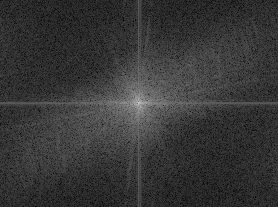
\includegraphics[width=2in]{images/origin_fft.png}}
  \caption{原图(1050px$\times$788px)及其傅里叶频谱图}
  \label{fig:origin} %% label for entire figure
\end{figure}

\begin{figure}[H]
  \centering
  \subfigure[图像]{
    \label{fig:blurred:a} %% label for first subfigure
    \includegraphics[width=2in]{images/blurred.bmp}}
  \hspace{1in}
  \subfigure[傅里叶频谱图]{
    \label{fig:blurred:b} %% label for second subfigure
    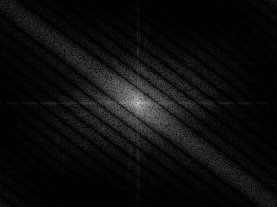
\includegraphics[width=2in]{images/blurred_fft.png}}
  \caption{运动模糊处理后 (尺度为20,角度为45)}
  \label{fig:blurred} %% label for entire figure
\end{figure}

\begin{figure}[H]
  \centering
  \subfigure[图像]{
    \label{fig:noisy:a} %% label for first subfigure
    \includegraphics[width=2in]{images/noisy.bmp}}
  \hspace{1in}
  \subfigure[傅里叶频谱图]{
    \label{fig:noisy:b} %% label for second subfigure
    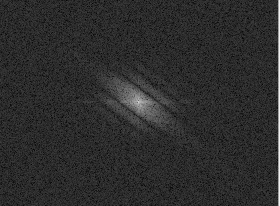
\includegraphics[width=2in]{images/noisy_fft.png}}
  \caption{运动模糊处理+噪音处理之后 (在前面的模糊图基础上加均值为1,方差为0.0001的高斯噪声后)}
  \label{fig:noisy} %% label for entire figure
\end{figure}

\subsection{直接逆滤波}

\begin{figure}[H]
  \centering
  \subfigure[对运动模糊图像还原]{
    \label{fig:direct:a} %% label for first subfigure
    \includegraphics[width=2in]{images/direct1.bmp}}
  \hspace{1in}
  \subfigure[对运动模糊+噪音图像还原]{
    \label{fig:direct:b} %% label for second subfigure
    \includegraphics[width=2in]{images/direct2.bmp}}
  \caption{使用直接逆滤波还原}
  \label{fig:direct} %% label for entire figure
\end{figure}

易见,使用直接逆滤波对无噪声的运动模糊图像进行还原时,其效果非常显著,图像的锐化程度进行了极大地提高。然而,当使用这种方法对只添加了少量高斯噪声的运动模糊图像进行还原时,还原后的图像可以说几乎完全无法直接读出原图像的信息,全图的像素均类似噪点。

\subsection{维纳滤波}

\begin{figure}[H]
  \centering
  \subfigure[对运动模糊图像还原]{
    \label{fig:weiner:a} %% label for first subfigure
    \includegraphics[width=2in]{images/weiner1.bmp}}
  \hspace{1in}
  \subfigure[对运动模糊+噪音图像还原]{
    \label{fig:weiner:b} %% label for second subfigure
    \includegraphics[width=2in]{images/weiner2.bmp}}
  \caption{使用维纳滤波器还原}
  \label{fig:weiner} %% label for entire figure
\end{figure}

使用维纳滤波对无噪声的运动模糊图像进行还原时,可以看出其效果与使用直接逆滤波的效果几乎相同,因为在这种情况下,维纳滤波与直接逆滤波对图像的处理是等价的。然而,当模糊图像出现了噪声时,还原后的图像尽管与无噪声的图像有些差距,但仍然较为清晰,锐化程度较高。

\section{运动模糊角度与尺度参数的估计}

\subsection{运动模糊角度的估计}

参考图\ref{fig:blurred:b}与图\ref{fig:noisy:b}。实际上,运动模糊图像的傅里叶频谱图有明显的暗线,暗线与x轴正方向的夹角就是图像模糊运动的角度逆时针旋转90°得到的。

因此,估算出傅里叶频谱图的暗线的角度,就可以大致测出拍摄图像时,物体与拍照设备的相对运动的角度。

\subsection{运动模糊尺度的估计}

估计出运动模糊角度,即可对运动模糊尺度进行估计。为了方便起见,我们先将图片旋转到模糊方向上,然后在图像中选取一小片图像样本,计算各行的自相关函数值$S_{x,y}$,将$S_{x,y}$各列求平均。结果即为水平方向上相关中心点两侧最低值点的距离。

\section{实验代码}
\begin{minted}{Matlab}
%Orignal Image
I = im2double(rgb2gray(imread('test.jpg')));
figure,subplot(3, 2, 1),imshow(I);
imwrite(I, 'origin.bmp');
title('1.原图');

temp = fft2(I);
temp = fftshift(temp);
temp = log(1 + abs(temp));
subplot(3,2,2),imshow(temp, []);
imwrite(temp, 'origin_fft.bmp');
title('2.原图的傅里叶频谱图');

%Blurred Image
PSF = fspecial('motion', 20, 45);
blurred_I = imfilter(I, PSF, 'conv', 'circular');
subplot(3, 2, 3), imshow(blurred_I);
imwrite(blurred_I, 'blurred_I.bmp');
title('3.运动模糊处理后的图(尺度为20,角度为45)')

temp = fft2(blurred_I);
temp = fftshift(temp);
temp = log(1 + abs(temp));
subplot(3,2,4),imshow(temp, []);
imwrite(temp, 'blurred_fft.bmp');
title('4.模糊图的傅里叶频谱图');

%Blurred Noisy Image
noise_mean = 0;
noise_var = 0.0001;
blurred_noisy_I = imnoise(blurred_I, 'gaussian', noise_mean, noise_var);
subplot(3, 2, 5),imshow(blurred_noisy_I);
imwrite(blurred_noisy_I, 'noisy.bmp');
title('5.在前模糊图基础上加均值为1,方差为0.0001之后的带噪点的模糊图');

temp = fft2(blurred_noisy_I);
temp = fftshift(temp);
temp = log(1 + abs(temp));
subplot(3,2,6),imshow(temp, []);
imwrite(temp, 'noisy_fft.bmp');
title('6.带噪点模糊图的傅里叶频谱图');

figure();

%Direct on Blurred Image
wnr1 = deconvwnr(blurred_I, PSF, 0);
subplot(2,2,1),imshow(wnr1);
imwrite(wnr1, 'direct1.bmp');

%Weiner on Blurred Image
wnr2 = deconvwnr(blurred_I, PSF, 0);
subplot(2, 2, 2), imshow(wnr2);
imwrite(wnr2, 'weiner1.bmp');

%Direct on Blurred and Noisy Image
wnr3 = deconvwnr(blurred_noisy_I, PSF, 0);
subplot(2, 2, 3), imshow(wnr3);
imwrite(wnr3, 'direct2.bmp');

%Weiner on Blurred and Noisy Image
signal_var = var(I(:));
wnr4 = deconvwnr(blurred_noisy_I, PSF, noise_var/signal_var);
imwrite(wnr4, 'weiner2.bmp');
subplot(2, 2, 4), imshow(wnr4);
subplot(2, 2, 3), imshow(wnr3);

\end{minted}
\section{结论}

通过理论分析,我们确实能够发现直接逆滤波器对有噪声的运动模糊图像的还原有很大的局限性,而通过实验,更加验证了这一想法。

而对于维纳滤波器,我们能够发现它的效果非常好,能够将模糊且有噪点的图像进行很大程度上的修复,使原图像的大部分细节得以重现。

\renewcommand\refname{参考文献}
\begin{thebibliography}{99}
\bibitem{art1} 周玉, 彭召意. 运动模糊图像的维纳滤波复原研究[J]. 计算机工程与应用, 2009, 45(19): 181-183.
\bibitem{book1} 奥本海姆, 谢弗, 巴克, 等. 离散时间信号处理: Discrete-time signal processing[M]. 西安交通大学出版社, 2001.
\bibitem{book2} 邓自立. 卡尔曼滤波与维纳滤波: 现代时间序列分析方法[M]. 哈尔滨工业大学出版社, 2001.

\end{thebibliography}

\end{document}
